\documentclass[border=10pt]{standalone}
\usepackage{pgfplots}
\pgfplotsset{compat=1.18}
\begin{document}
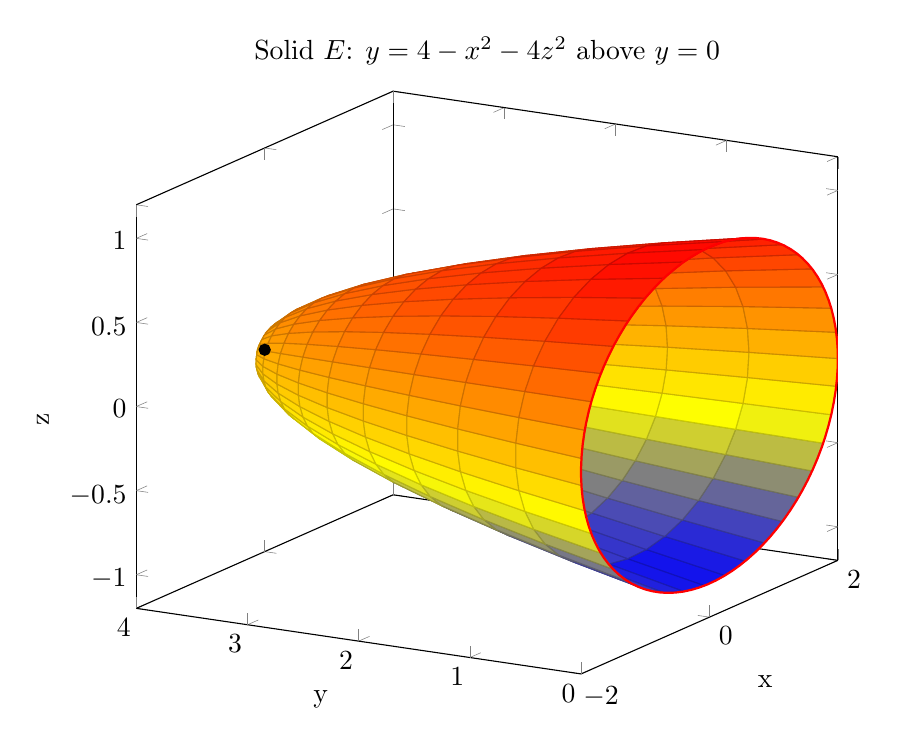
\begin{tikzpicture}
\begin{axis}[
    view={-60}{18},
    xlabel={x}, ylabel={y}, zlabel={z},
    title={Solid $E$: $y=4-x^2-4z^2$ above $y=0$},
    scale=1.3
]
% Paraboloid surface parametrized by (2r cos t, 4 - 4r^2, r sin t)
\addplot3[
    surf,
    shader=faceted,
    domain=0:360, samples=40,
    y domain=0:1, samples y=12,
    z buffer=sort
] ({2*y*cos(x)}, {4 - 4*y*y}, {y*sin(x)});
% Base ellipse on y=0
\addplot3[domain=0:360, samples=100, samples y=0, red, thick]
    ({2*cos(x)}, {0}, {sin(x)});
% Vertex point
\addplot3[only marks, mark=*, mark size=2pt, black] coordinates {(0,4,0)};
\end{axis}
\end{tikzpicture}
\end{document}